\chapter{Etapas de Desenvolvimento e Implementação}
\label{ch::imp-test}

\section{Introdução}
\label{sec::imp-test:intro}

Para o sucesso deste projeto foi essencial delinear uma estratégia de investigação. Esta divide-se em 3 partes: reconstrução dos hologramas, compressão dos hologramas reconstruídos, e determinação das métricas de compressão. A cada uma destas fases atribuíram-se objetivos para a sua profícua execução:

\begin{enumerate}
    \item Reconstrução dos hologramas:
    \begin{enumerate}
        \item Estudar a holografia;
        \item Estudar as funções originais em MATLAB do Projecto JPEG Pleno;
        \item Transcrever estas funções para a linguagem de programação Python;
        \item Comparar o \textit{output} entre as funções originais em MATLAB e as respetivas transcrições em Python;
        \item Desenvolver um \textit{script} para reconstruir cada holograma em 16 vistas distintas.
    \end{enumerate}

    \item Compressão dos hologramas reconstruídos:
    \begin{enumerate}
        \item Estudar o uso do \ac{kdu};
        \item Automatizar a execução dos \textit{scripts} e \textit{softwares} envolvidos;
        \item Implementar um \textit{script} para compressão (com e sem transformada de cor em diferentes \textit{bitrates}) e descompressão dos hologramas reconstruídos.
    \end{enumerate}

    \item Determinação das métricas de compressão:
    \begin{enumerate}
        \item Calcular o débito com a métrica \ac{PSNR} entre os hologramas originais e as imagens comprimidas;
        \item Determinar o melhor método de armazenamento dos débitos calculados;
        \item Implementar o \textit{output} dos resultados no método selecionado;
        \item Gerar gráficos dos resultados.
    \end{enumerate}
\end{enumerate}

As Secções subsequentes expõem o trabalho desenvolvido neste sentido e a Figura \ref{fig:projeto} esquematiza o processo levado a cabo para a execução do projeto.

\begin{figure}[!htbp]
    \centering
    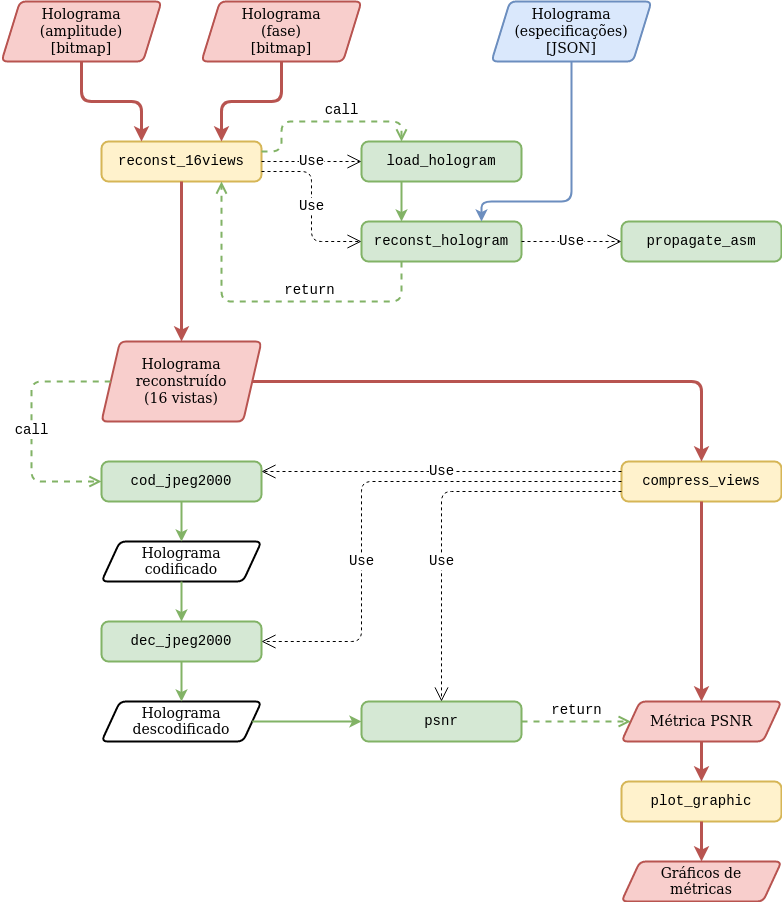
\includegraphics[width=\textwidth]{projeto}
    \caption
        [Diagrama do processo efetuado sobre um holograma para obtenção dos resultados.]
        {
            Diagrama do processo efetuado sobre um holograma para obtenção dos resultados.\\
            O caminho vermelho/amarelo representa o trajeto principal pelo qual o holograma sofre processamento. Os caminhos verdes detalham os processos intermédios correspondentes a um determinado processo do trajeto principal (a entrada é dada por ``\textit{call}'' e o retorno é dado por ``\textit{return}''). As dependências entre as principais funções são indicadas por ``\textit{Use}''. A azul estão os ficheiros externos auxiliares. \\
        }
    \label{fig:projeto}
\end{figure}


\section{Reconstrução dos Hologramas}
\label{sec::imp-test:reconst-hologram}
% [X] Estudo holografia
% [X] estudo funções matlab
% [X] transcrever funções para scripts em python
% [X] comparar output entre funções de matlab e python para confirmar que os hologramas estão a ser reconstruídos corretamente
% [X] desenvolver script para reconstruir o mesmo holograma de 16 vistas diferentes

O projeto iniciou-se com uma pesquisa exaustiva sobre a ciência da holografia, a qual resultou no Estado da Arte resumido no Capítulo \ref{ch::estado-arte}.

Simultaneamente, foi efetuado um estudo das funções do \textit{software} desenvolvido no âmbito do projeto JPEG Pleno a fim de se poder fazer a respetiva transcrição para Python. O resultado deste estudo e transcrição encontra-se exposto nas tabelas \ref{tab:load_hologram}, \ref{tab:propagate_asm} e \ref{tab:reconst_hologram}.

Estas funções foram compiladas num único \textit{script} Python. A fim de cumprir o \ref{obj:reconstruir_vistas}\textordmasculine~objetivo secundário, uma nova função, \verb|reconst_16views|, foi implementada (Tabela \ref{tab:reconst_16views}). Esta função está, portanto, encarregue de abrir um holograma, as respetivas especificações e reconstruí-lo em exatamente 16 vistas distintas. De notar que as especificações são fornecidas por um ficheiro \ac{JSON} cujo conteúdo inclui:
\begin{itemize}
    \item \verb|holo_size|: Resolução do holograma (em pixeis);
    \item \verb|pitch|: Distância entre pixeis (em metros);
    \item \verb|wavelenghts|: Lista com os comprimentos de onda respetivos aos canais \ac{RGB} (em metros);
    \item \verb|z|: Distância de reconstrução (em metros);
    \item \verb|pupil_size|: Lista que contém o tamanho da janela de reconstrução (em pixeis).
\end{itemize}

\begin{figure}[!htbp]
    \centering
    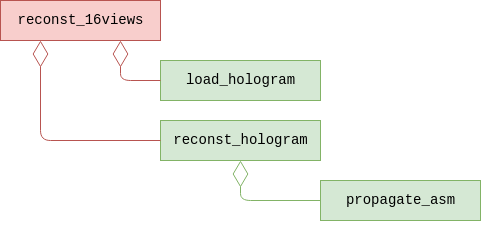
\includegraphics[scale=.6]{reconst_16views}
    \caption{Diagrama de dependências da função \texttt{reconst\_16views}.}
    \label{fig:reconst_16views}
\end{figure}

Todavia, havendo uma transcrição de funções entre linguagens de programação, exigiu-se uma forma de comprovar que as funções transcritas em Python são equivalentes às originais em MATLAB. Para este fim, delineou-se a seguinte estratégia:

\begin{enumerate}
    \item Etapa de implementação:
    \begin{enumerate}
        \item Transcrever as funções para Python (forme apresentado).
    \end{enumerate}
    
    \item Etapa de reconstrução:
    \begin{enumerate}
        \item Reconstruir os hologramas numa vista com as funções originais em MATLAB;
        \item Reconstruir os hologramas numa vista com as funções transcritas em Python.
    \end{enumerate}

    \item Etapa de comparação e resultados:
    \begin{enumerate}
        \item Comparar os hologramas produzidos pelos \textit{scripts} das duas linguagens através de uma análise visual a olho nu;
        \item Comparar os hologramas produzidos pelos \textit{scripts} das duas linguagens através da métrica \ac{PSNR}.
    \end{enumerate}
\end{enumerate}

Com o \textit{script} devidamente implementado e testado, prosseguiu-se com a seguinte fase do projeto relativo à compressão dos hologramas agora reconstruídos.


\section{Compressão dos Hologramas Reconstruídos}
\label{sec::imp-test:holo-compress}
% [X] estudar o uso de kdu
% [X] automatização de execução dos softwares
% [X] implementar script que comprime com e sem transformada de cor, e com bitrates: [0.1, 0.3, 0.6, 1.0, 1.5, 2.0, 2.5, 3.0, 3.5, 4.0, 4.5, 5.0], e descomprime as reconstruções do holograma

Após a reconstrução dos hologramas em multivista, segue-se o teste ao formato JPEG2000 através de compressão e descompressão de forma a comparar com a reconstrução do holograma original (cuja métrica será abordada na Secção \ref{sec::imp-test:psnr}).

Conforme a estratégia delineada na Secção \ref{sec::imp-test:intro}, esta fase do projeto envolveu o estudo da ferramenta \ac{kdu}, a implementação dos \textit{scripts} e o cálculo das métricas.

\subsection{Breve Estudo do \textit{Kakadu Software}}
\label{ssec::imp-test:holo-compress:estudo-kdu}

A fase de estudo do \ac{kdu} resultou no conhecimento exposto na Secção \ref{ssec::tecno-ferr:tecno-ferr:kdu}, onde se encontram descritos os dois comandos utilizados no âmbito do projeto.


\subsection{Implementação e Execução do \textit{Script} de Compressão}
\label{ssec::imp-tes:holo-compress:script}

De forma a se poder comparar o holograma original com o holograma comprimido no formato JPEG2000, revela-se necessário realizar uma sequência de compressão e descompressão do primeiro. Tal irá dar origem a um holograma reconstruido após compressão, o qual poderá ser comparado com o original.

Conforme visto anteriormente, a ferramenta \ac{kdu} é a ferramenta eleita para este processo. Contudo, não é prático executar manualmente a sequência de comandos na \textit{shell}. Por conseguinte, um \textit{script} escrito em Python foi implementado. Este inclui a função \verb|compress_views| (Tabela \ref{tab:compress_views} e Figura \ref{fig:compress_views}), a qual executa a seguinte sequência de operações:

\begin{enumerate}
    \item \textit{Compressão do holograma original, previamente reconstruido.} \\
        É feita uma chamada ao sistema do comando \verb|kdu_compress|.\\ Esta encontra-se encapsulada na função auxiliar \verb|cod_jpeg2000| (Tabela \ref{tab:cod_jpeg2000}).
    \item \textit{Descompressão do holograma agora comprimido.} \\
        É feita uma chamada ao sistema do comando \verb|kdu_expand|.\\ Esta encontra-se encapsulada na função auxiliar \verb|dec_jpeg2000| (Tabela \ref{tab:dec_jpeg2000}).
    \item \textit{Cálculo do débito através de uma métrica de compressão.} \\
        O holograma original e o holograma agora descomprimido são comparados com recurso à métrica \ac{PSNR} (Secção \ref{sec::imp-test:psnr}).\\ Esta operação é realizada pela função auxiliar \verb|psnr| (Tabela \ref{tab:psnr}).
\end{enumerate}

De notar os \textit{bitrates} testados: \SI{0.1}{}, \SI{0.3}{}, \SI{0.6}{}, \SI{1.0}{}, \SI{1.5}{}, \SI{2.0}{}, \SI{2.5}{}, \SI{3.0}{}, \SI{3.5}{}, \SI{4.0}{}, \SI{4.5}{} e \SI{5.0}{}. Há ainda a referir a realização dos testes com e sem transformada de cor.

\begin{figure}[!htbp]
    \centering
    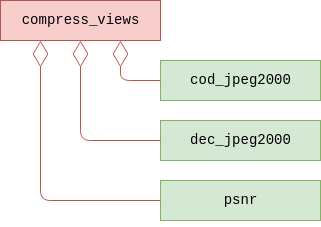
\includegraphics[scale=.6]{compress_views}
    \caption{Diagrama de dependências da função \texttt{compress\_views}.}
    \label{fig:compress_views}
\end{figure}

Por fim, de forma a facilitar a extração dos resultados pretendidos segundo o objetivo primário do projeto (Secção \ref{sec::intro:objs}), é gerado um ficheiro \ac{JSON} por cada holograma. Este tem a seguinte estrutura:

\begin{figure}[!h]
\dirtree{%
    .1 <nome\_holograma>.json.
    .2 no\_ycbcr.
    .3 <rate>\DTcomment{\small Número de \textit{bits} por amostra}.
    .4 <vista>.ppm: valor\DTcomment{\small Posição da janela de reconstrução}.
    .4 avg: valor\DTcomment{\small \ac{PSNR} médio das vistas para este \textit{rate}}.
    .4 std: valor\DTcomment{\small Desvio padrão}.
    .2 ycbcr.
    .3 <rate>.
    .4 <vista>.ppm: valor.
    .4 avg: valor.
    .4 std: valor.
}
\end{figure}

O ficheiro \ac{JSON} supra-mencionado será portanto utilizado no processo descrito na Secção \ref{sec::imp-test:psnr}.


\subsection{Automatização dos \textit{Scripts}}
\label{ssec::imp-test:holo-compress:auto-script}

Para a otimização do processo de investigação neste projeto, foram criados dois \textit{scripts} adicionais, os quais trabalham em conjunto a fim de automatizar todo este processo. São eles os seguintes:
\begin{enumerate}
    \item \textit{Makefile}: Introduz as 8 opções infra-apresentadas, as quais invocam o \textit{script} \verb|main.py|: 
        \begin{enumerate}
            \item \verb|reconst|: reconstrói o holograma fornecido por argumento em 16 vistas (Capítulo \ref{sec::imp-test:reconst-hologram} e Tabela \ref{tab:reconst_16views});
            \item \verb|compress|: executa o \textit{script} apresentado na Secção \ref{ssec::imp-tes:holo-compress:script};
            \item \verb|plot|: calcula os gráficos com os resultados de comparação da   compressão com e sem transformada de cor (Secção \ref{sec::imp-test:psnr});
            \item \verb|all|: executa os 3 itens anteriores;
            \item \verb|test|: opção utilizada na fase de \textit{debugging};
            \item \verb|install|: instala pacotes no sistema operativo essenciais à execução dos \textit{scripts};
            \item \verb|clean|: remove os diretórios relativos a: hologramas reconstruidos, \textit{output} do \ac{kdu}, ficheiros \ac{JSON} dos resultados do \ac{PSNR}, e ficheiros de \textit{cache} do Python;
            \item \verb|clean-compressed|: remove os diretórios relativos a: \textit{output} do \ac{kdu}, ficheiros \ac{JSON} dos resultados do \ac{PSNR}, e ficheiros de \textit{cache} do Python.
        \end{enumerate}
    \item \verb|main.py|: \textit{script} Python que executa as primeiras 5 opções supra-mencionadas conforme o argumento passado pelo \textit{Makefile}. Faz uso das funções \verb|reconst_16views| (Tabela \ref{tab:reconst_16views}) e \verb|compress_views| (Tabela \ref{tab:compress_views}).
\end{enumerate}


\section{Determinação das Métricas de Compressão}
\label{sec::imp-test:psnr}

% [X] calcular o débito com a métrica PSNR entre o holograma original e a imagem comprimida
% [X] estudar qual a melhor forma de guardar os débitos calculados
% [X] implementar no script a escrita dos dados num ficheiro json
% [X] a partir dos ficheiros json gerados, criar gráficos para apresentar os resultados com uso da biblioteca matplotlib.pyplot

Na sequência do processo de compressão e descompressão no formato JPEG2000, e conforme previamente introduzido na Secção \ref{ssec::imp-tes:holo-compress:script}, a determinação das métricas de compressão constituem a última fase da investigação a fim destes resultados poderem ser escrutinados no Capítulo \ref{ch::test-result}.

Variadas métricas estão disponíveis para se poder comparar amostras e, no caso do presente projeto, avaliar a qualidade do holograma após compressão no formato JPEG2000. De entre as métricas existentes, foi eleita a \acf{PSNR} por indicação da professora orientadora, a qual está envolvida no Projeto JPEG Pleno.

Conforme introduzido na Secção \ref{ssec::imp-tes:holo-compress:script}, foi utilizada uma função auxiliar \verb|psnr| (Tabela \ref{tab:psnr}), invocada pela função principal \verb|compress_views| (Tabela \ref{tab:compress_views}). Este método de implementação foi escolhido para fins de eficiência de armazenamento.

Uma vez que não é mandatório armazenar os hologramas rescontruídos após compressão, sendo apenas do nosso interesse as métricas finais a si referentes, a função \verb|dec_jpeg2000| exporta o holograma descomprimido num ficheiro temporário \verb|temp.ppm|. Este é utilizado de seguida pela função \verb|psnr| para cálculo do \ac{PSNR} (sendo os resultados armazenados num ficheiro \ac{JSON}), sendo de seguida eliminado.


\subsection{Criação de gráficos}
\label{ssec::imp-test:psnr:graf}

O ficheiro \ac{JSON} gerado (descrito na Secção \ref{ssec::imp-tes:holo-compress:script}) é posteriormente carregado num novo \textit{script} Python, especificamente implementado para gerar gráficos em si baseados para mais fácil visualização, análise e discussão (Capítulo \ref{ch::test-result}). Este \textit{script} recorre à biblioteca \verb|matplotlib.pyplot|.

A geração de um gráfico por holograma por parte deste \textit{script} marca o fim do processo de investigação relativo à manipulação dos hologramas e extração de métricas.


\section{Conclusões}
\label{sec::imp-test:conclusao}

Após a conclusão das 3 fases de investigação segundo a estratégia delineada inicialmente e ilustrada pela Figura \ref{fig:projeto}, resta a exposição e análise dos resultados obtidos no Capítulo \ref{ch::test-result}.

A estratégia desenhada revelou-se eficaz e permitiu a obtenção de \textit{scripts} facilmente adaptáveis para trabalhos futuros no âmbito do Projeto JPEG Pleno, assim como os próprios resultados para análise por parte de outros interessados. De igual forma, a escolha de \textit{standards} gratuitos e \textit{open-source} (justificada na Secção \ref{sec::tecno-ferr:tecno-ferr}) revelou-se acertada pelos mesmos motivos.

